\documentclass[10pt]{beamer}

%\usepackage[utf8x]{inputenc}
\usepackage{ngerman}
\usepackage[ngerman]{babel}
\usepackage{amsmath}
\usepackage{bbm}

\usepackage{tabularx}
\usepackage{graphicx}
\usepackage{subfigure}
\usepackage{url}
%\usepackage{hyperref}
\usepackage{eurosym}
\usepackage{listings}

\usepackage{multirow}
\usepackage{colortbl}
\usepackage{booktabs}
\usepackage{setspace}

\input{theme/theme}

\title{Linux Cluster in Theorie und Praxis}
\subtitle{Insert your title here}
\author{Christian Deussen}
\date{10. Februar 2015}
\institute[ZIH TUD]{Zentrum f\"ur Informationsdienste und Hochleistungsrechnen -- TU Dresden}
%\room{INF 1046}
\address{N\"othnitzer Stra{\ss}e 46}
\city{01189 Dresden}
%\phone{+49 0351 - 463 38783}
\email{s3066193@mail.zih.tu-dresden.de}

\setbeamercovered{transparent}
\begin{document}

\zihmaketitle

\begin{frame}
\frametitle{Inhalt}
 \tableofcontents
\end{frame}


\section{Mean Shift}
\begin{frame}
	\frametitle{Einf\"uhrung}
	\includegraphics[scale=0.34, keepaspectratio]{pics/s1_black.png}
	\includegraphics[scale=0.34, keepaspectratio]{pics/s1_colored.png}
\end{frame}
\begin{frame}
	\frametitle{Einf\"uhrung}
\end{frame}

\section{Implementation}
\begin{frame}
	\frametitle{MPI Implementation}
	\begin{itemize}
		\item Insert your content
	\end{itemize}
\end{frame}

\section{Benchmarks}
\begin{frame}
	\frametitle{Cluster Benchmark}
	\begin{itemize}
		\item Insert your content
	\end{itemize}
\end{frame}

\section{Beispiele}
\begin{frame}
	\frametitle{Einf\"uhrung}
	\includegraphics[scale=0.34, keepaspectratio]{pics/s2_black.png}
	\includegraphics[scale=0.34, keepaspectratio]{pics/s2_colored.png}
\end{frame}
\begin{frame}
	\frametitle{Einf\"uhrung}
	\includegraphics[scale=0.34, keepaspectratio]{pics/s3_black.png}
	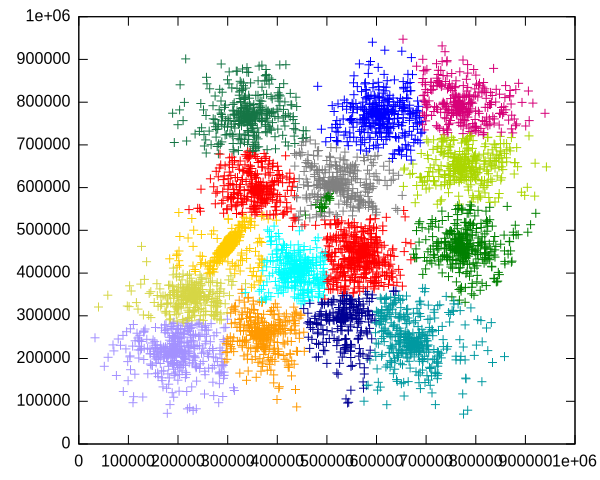
\includegraphics[scale=0.34, keepaspectratio]{pics/s3_colored.png}
\end{frame}
\begin{frame}
	\frametitle{Einf\"uhrung}
	\includegraphics[scale=0.34, keepaspectratio]{pics/s4_black.png}
	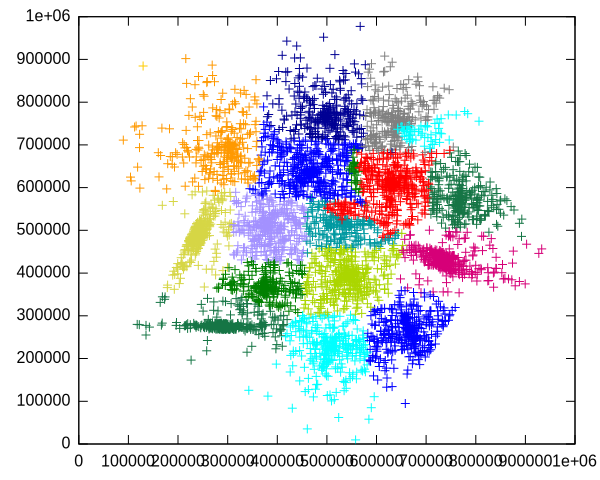
\includegraphics[scale=0.34, keepaspectratio]{pics/s4_colored.png}
\end{frame}
\end{document}
